\documentclass[12pt]{article}

\usepackage{graphicx}
\usepackage{manfnt}
\usepackage{hyperref}

\setlength{\oddsidemargin}{0cm}
\setlength{\evensidemargin}{0cm}
\setlength{\topmargin}{0cm}
\setlength{\textwidth}{16cm}
\setlength{\textheight}{22cm}
\begin{document}
\begin{center}
\Huge User manual for Ortho4XP\\
\large version 1.11 released\\
\Large January 19th 2016
\end{center}

\tableofcontents

\section{Introduction}
Ortho4XP is a cross-platform open source tool whose primary aim is to build orthophotos based sceneries for the X-Plane 10 flight simulator at the cost of a few mouse clicks. The building process is not based on existing sceneries or meshes, neither on Laminar's Meshtool, but instead relies exclusively on :
\begin{itemize}
  \item {\bf Openstreetmap} for information regarding airports, coastline, rivers, lakes, docks etc.
  \item {\bf Elevation files} whose data is used to construct altitudes but also to adapt mesh density to local terrain complexity.
  \item {\bf Tile Map Services (TMS)} which serve as providers for the orthophotos\footnote{The copyrights regarding these services should be considered seriously. Fortunately the majority of them tolerate private non commercial ``fair'' use, and an increasing number of them are even going open data. The INSPIRE European rule is a really nice move in that direction.}.
\end{itemize}

The DSF files produced by Ortho4XP contain {\it only} the bottom layer of the X-Plane scenery hierarchy : a base mesh, that is a set of textured 3D triangles covering the whole tile\footnote{Strictly speaking transparency water effects are obtained by a combination of base triangles of X-Plane water type with overlay masked triangles textures with orthophotos.}.
In particular, information such as road networks, forest polygons, buildings, and more generally anything which is an overlay over the mesh is {\it not} part of the Ortho4XP todo list.
There are very good third party resources for the later which complement perfectly and {\it without intersection}\footnote{Even though X-Plane deals pretty well with the abundance of repetitive information through its exclusion processes, it also certainly influences its load time at least.} with Ortho4XP, in particular World2XPlane and/or local sceneries.

Besides the basic features related to download and attribution of textures, one can list the following regarding the building process and/or its output :
\begin{enumerate}
  \item A graphical interface that allows to select different zones with different zoomlevels and/or providers directly inside the software.
  \item A user controlled global mesh complexity, which covers the range between the stock global scenery and ultra high density meshes, actually way beyond, with only a limited impact on runtime.
  \item Transparency/blending effects for inland and sea water. The first through a configurable alpha channel ratio, and the second through the automatic generation of blured alpha masks following the coastline.
  \item Every airport whose boundary is defined in Openstreetmap is automatically flattened along its boundary.
  \item The ability to patch the mesh at the very early stage of the building process, in particular to easily burn in well rounded sloped runways, or to flatten specific areas at a fixed altitude.
\end{enumerate}


\section{Installation}

The installation of Ortho4XP {\it per se} is only a matter of decompressing the included 7z archive to your prefered location on disk.
Keep in mind that orthophotos based sceneries are demanding in terms of file size, and therefore it is presumably a good idea to choose a partition with a comfortable amount of free space.
Also, on Linux and OS X you should check after decompression of the archive that the files {\tt Ortho4XP.py} and {\tt Utils/Triangle4XP} (Linux) or {\tt Utils/Triangle4XP.app} (OS X) have the appropriate execution rights. In case not, these can be recovered issuing {\tt chmod a+x Ortho4XP.py} for the first one, and {\tt chmod a+x Utils/Triangle4XP} for the second.

\medskip

The {\bf evil} before you can start building tiles is hidden in the fact that Ortho4XP is {\it not} a standalone software. It requires a number of (open source) software packages as prerequisites. Note however that you won't need to use them directly, but Ortho4XP will.
These are :

\begin{itemize}
  \item A Python 3 interpreter along with the following extra Python modules: {\it requests}, {\it numpy}, {\it overpy}, {\it tk} and (optional) {\it gdal} and {\it pyproj}.
  \item Imagemagick (for convert and montage command-line tools), version $>=$ 6.8 preferred.
  \item nvtools nvcompress -the NVidia Tools Extension (provides a cross platform dds library)
\end{itemize}
To be able to use Ortho4XP to its full extent the following additional software should be present as well :
\begin{itemize}
  \item Gimp and/or Netpbm (process times being shorter with the first of these two).
\end{itemize}

Whatever the way you follow to install these prerequisites (in particular the ones outlined in the README.install), you are strongly encouraged to perform the following tests after installation to check whether everything is in order :

\begin{enumerate}
  \item Fire up your Python 3 interpreter, e.g. through a command terminal window.\\
  \hspace*{-1cm}\dbend\hspace*{0.3cm}(check that you indeed launched Python 3, not e.g. version 2.7 which may coexist alongside on many systems)
  \item At the Python prompt issue {\tt import requests, overpy, numpy, tk}.\\
  You should only obtain a new command prompt and no error messages.
  \item Do the same with the command {\tt from PIL import ImageTk}.\\ 
  Here again you shouldn't obtain anything more than a new command prompt.
  \item Exit the Python interpreter (e.g. with the command {\tt quit()}).
  \item In a command terminal window of your OS, issue {\tt convert -list format} (or
  {\tt convert.exe -list format} if on Windows). You should obtain a (long sorted) list of delegates available to Imagemagick, and {\tt DDS* DDS rw+ Microsoft DirectDraw Surface} should be one of those.
\end{enumerate}

If you additionally wish to be able to automatically build transparency masks for coastlines (or so-called {\it sea\_equiv} user-defined regions), you should succeed in at least one of the following two tests :
\begin{enumerate}
  \setcounter{enumi}{5}
  \item Netpbm is present on your computer and possesses the executable {\tt pamundice} (other required executable are assumed to be present if {\tt pamundice} is).
  \item Gimp is present on your computer and issuing the command\\
  {\tt gimp -i -c -b '(blurX "test.png" 16 "result.png")' -b '(gimp-quit 0)'}\\
  from within a terminal window in the directory ~/Utils should produce a png file called result.png in that same directory, which can be opened with an image viewer.\\
  \hspace*{-1cm}\dbend\hspace*{0.3cm} You will most probably need to copy the file {\tt blurX.scm}, found in the directory Utils, to the script-fu directory of your Gimp install (e.g. {\tt \$HOME/.gimp-2.8/scripts/} on Linux and Max OS X).
\end{enumerate}
If you succeeded in installing the preceding prerequisites, congratulations, you may now embark in using Ortho4XP !

\section{First test tile in Brittany}

In this section we shall follow step by step the creation of a first tile using only basic features.
The tile corresponds to the Ouessant island in the extreme west of Brittany in France. Since the land cover of that tile is small, the whole process shouldn't take longer than a couple of minutes (in addition to the ones you'll be employing reading these notes carefully of course!).

We begin by launching the application Ortho4XP (the heart of the application is the source file Ortho4XP.py). Depending on your system and the file associations which you have configured, you may simply have to double-click the file Ortho4XP.py in a file browser (prefered way), or else to issue the command {\tt python3 ./Ortho4XP.py} (Linux, OS X) or {\tt py.exe -3 Ortho4XP.py} (Windows), possibly replacing the Python interpreter name depending on your exact set-up.

We are now in front of the main window (Figure \ref{fig:main_window}). At the top of that window, we can read the latitude and longitude coordinates of the tile to be built (these follow the same rules as X-Plane, i.e. they correspond to the coordinates of the point at the south west corner of the tile). For this first tile, we will leave the default values 48 -6 which indeed correspond to the Ouessant island. We will also leave the {\tt custom build\_dir} checkbox unchecked, so that we will construct the tile within the default (and newly created) directory called {\tt zOrtho4XP\_+48\_-006} (within the main Ortho4XP dir).
\begin{center}
\begin{figure}[!ht]
\begin{center}
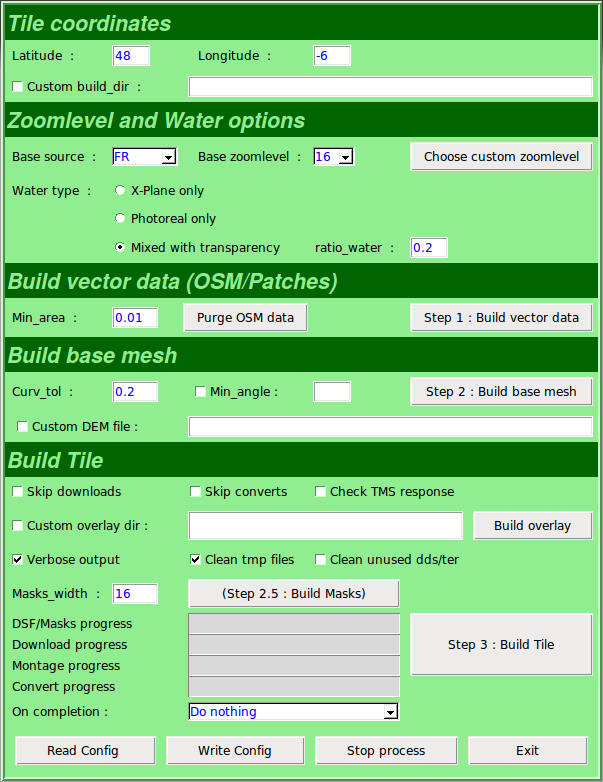
\includegraphics[width=14cm]{Images/main_window.png}
\caption{\label{fig:main_window}Main window (croped)}
\end{center}
\end{figure}
\end{center}

\medskip

We step forward to the ``Zoomlevel and Water options" section. The base provider and base zoomlevel for the tile are given in the first two listboxes. Since Ouessant is only 6 squared miles, we can safely increase the base zoomlevel to, say, 18, whereas for the provider we shall choose the local 'FR' source, but the default 'BI' would be a very good choice too. We shall not define additional custom zoomlevels for this first tile, and stick to the ``Mixed with transparency" water option which is certainly the nicest one (the other two are left either for very low end configurations or for specific tasks not described here).

The parameter {\tt ratio\_water} is related to the proportion of ``X-Plane water'' in its blending process with water from orthophotos, only for {\bf inland} water. For the present tile, that will only apply to two small patches of water right in the middle of the island, and is therefore not of the utmost importance. The default value can actually be considered a good value for {\it any} tile, but that may depend on user taste.

\medskip

Now comes the first real step, in section ``Build vector data (OSM/Patches)'', where we will download all vector data related to boundaries of ground with water as well as of airports from Openstreetmap.
The parameter {\tt Min\_area} represents a surface in square kilometers: Every single closed loop of water whose surface is less than this value will be discarded in the building process. In principle one could simply set it to $0$, to get the full Openstreetmap data. In practice, this is not always the best option because this can imply a higher complexity for the mesh while transparency effects become barely visible whith decreasing surface area. For this first example we can safely take it to be $0$ though.

Check that your internet connection is working and click (once!) on the button ``Step 1 : Build vector data''.
The right terminal pane of the window should start to animate itself and you'll get information on the process until completion indicating process time. For Ouessant, this shouldn't take much more than a few seconds.

\medskip

Before we jump to Step 2, let us have a look at Figure \ref{fig:poly} showing the vector data that we have just processed (contained in {\tt Data+48-006.poly} in the folder {\tt zOrtho4XP\_+48-006} below the main Ortho4XP directory).
\begin{center}
\begin{figure}[!ht]
\begin{center}
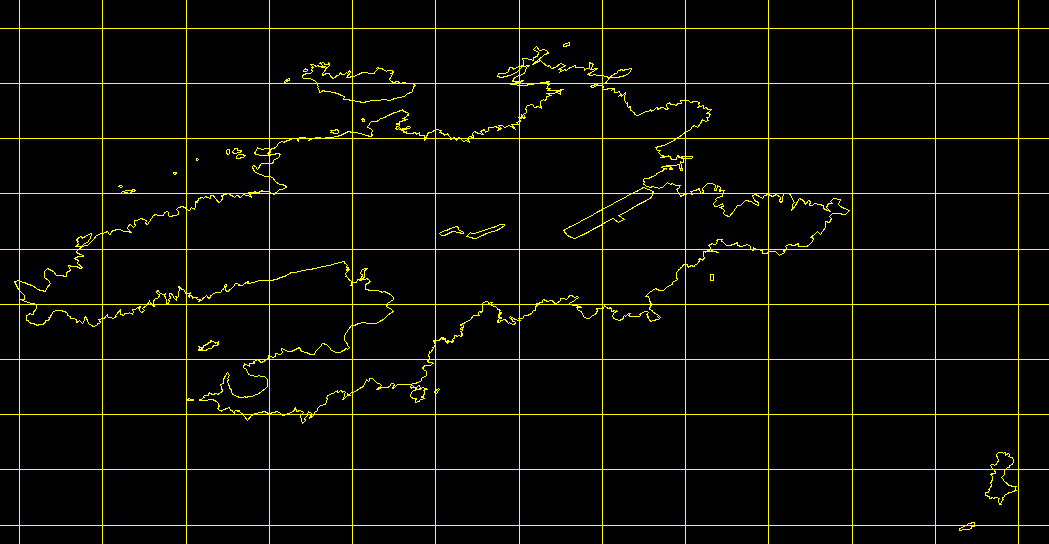
\includegraphics[width=14cm]{Images/ouessant_poly.png}
\caption{\label{fig:poly}Vector data (croped around the island)}
\end{center}
\end{figure}
\end{center}
Besides the coastline, one can see the boundaries of LFEC airport (east), the two patches of inland water (center), and of course the grid, which corresponds to the trace cut of potential ZL19 orthophotos (even though we will not use such high zoomlevels here, the mesh will be ready to support them).

\medskip

In Step 2, we have to decide a value for the parameter {\tt Curv\_tol}. It is very important to understand the meaning and the importance of that parameter, which is related to the complexity of the mesh to be created. Its acronym stands for ``tolerance to curvature'', and therefore the higher it is, the higher tolerance is, and the lower mesh complexity will be. When a terrain is bumpy, it requires a higher density of mesh points to approximate it within a certain tolerance, with respect to a flat terrain.
The parameter {\tt Curv\_tol} controls how far in the refinement the mesh algorithm will go to approximate the mesh to reality. In regions which are not terrifically bumpy as in Ouessant, a low value, such as as say $0.2$, can be used to get a fine approximation. In the mountains like e.g. the +45+006 tile, a higher value of $3$ will already give a very complex mesh, and a value of $0.2$ there would certainly lead to a mesh way too heavy (and which will actually fail to be transformed into a dsf). There is no black magic here, and you''ll surely quickly get acquainted with this parameter.
Also, we will get information regarding our mesh complexity, and the possibility to revert to different values of the parameter as many times as we please, after we launch the Step 2 button right now:

\begin{center}
\begin{figure}[!ht]
\begin{center}
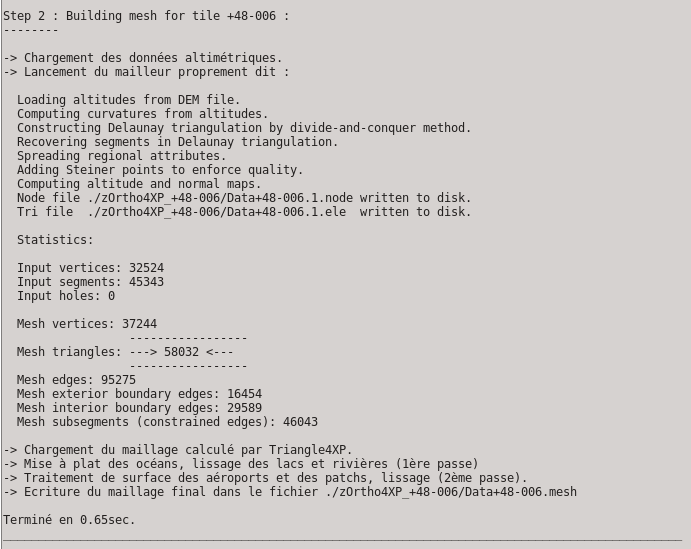
\includegraphics[width=14cm]{Images/ouessant_step2.png}
\caption{\label{fig:text_step2}Outcome of Step 2 in this example}
\end{center}
\end{figure}
\end{center}

As we can see, our mesh has 58032 triangles. This is not a lot in absolute value, compared to the global scenery tiles of X-Plane that have something like 500.000 triangles.  Or course this has to be put in relation with the size of the island. In the next figure we can have a closer look at the triangles of the mesh (file Data+48-006.1.ele). To get an idea of their size, keep in mind that any box of the grid is roughly 800m of lateral size (this actually varies depending on latitude), so that triangles here range somewhere between 20m for the smallest and 200m for the largest (and even 800m for those fully offshore).
What we can observe as well is that the vector data of Step 1 is present as so-called ``required-edges'', meaning that they are part of the triangles edges, and the latter therefore do not have transverse intersection with the vector data (in straight terms: the mesh respects the terrain boundaries).

\begin{center}
\begin{figure}[!ht]
\begin{center}
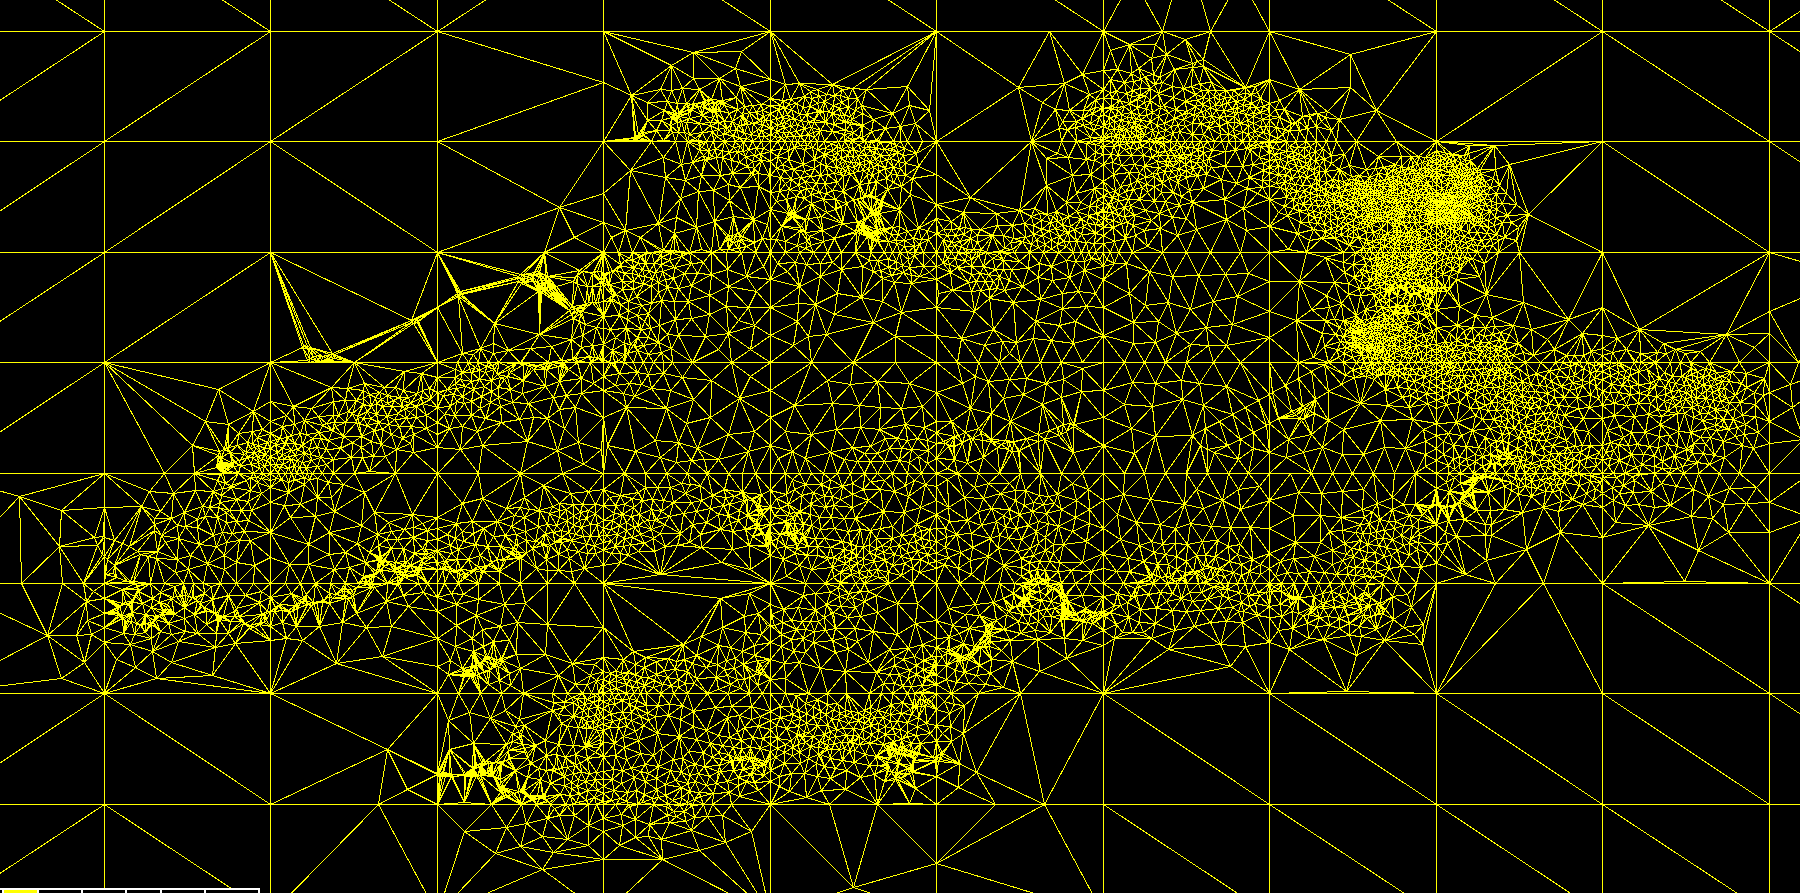
\includegraphics[width=16cm]{Images/ouessant_step3.png}
\caption{\label{fig:plot_step2}Mesh density}
\end{center}
\end{figure}
\end{center}

As we can see also, a small proportion of the triangles have a pretty small smallest angle. This is generally something that people working with meshes try to avoid, in particular when computations need to be done with those meshes.
Within X-Plane, there is not quite such a rule, but in specific cases that may help and that is the goal of the checkbox {\tt Min\_angle} which we haven't used here (its usefulness is mainly in order when dealing with the more advanced feature of - Patches - or user-customized local mesh).
Furthermore, you could ask yourself where the elevation data that the mesh algorithm has been using came from. In this specific case, it turns out that the elevation file for the +48-006 tile is included (and this is the only one) in the 7z archive coming along Ortho4XP. This file is located in the directory {\tt Elevation\_data}, which is the default location where the software is looking for them, unless we specify something different in the {\tt Custom DEM\_file} file chooser.

We are ready to proceed to the last step, and since we wish to avoid a harsh transition between the land of the island and the sea, we shall build transparency masks. Basically, these are b\&w png files which will eventually serve as BORDER TEX in X-Plane's terrain files, and which are obtained in the following way : first a binary black and white image is constructed from the information of the mesh, with white pixels for ground and black ones for water. These are then blured according to the blur radius indicated in the {\tt Masks\_width} entry, and then leveled up for artistic purposes. In rough terms, one pixel of blur radius corresponds to 10m of offshore data.
The higher the {\tt Masks\_width} the smoother the transition, but we are limited by the location over the sea where orthophotos starts to look bad (typically completely white or a plain saturated blue).
In Ouessant and with the 'FR' provider, we can safely ask for a Masks\_width of 32. We push the ``(Step 2.5 : Build Masks)'' button and wait for completion. If you are relying on Gimp the process will be fast (under one minute), whereas the combination Imagemagick/Netpbm will need almost an order of magnitude longer (we are dealing with images that are approximately 600 Mpix in size...).
In any case, keep in mind that process time is somehow proportional to the value of Masks\_width.

Finally, we push the ``Step 3 : Build Tile'' button and wait for completion. Once finished, the directory {\tt zOrtho+48-006} can be used directly within the {\tt Custom Scenery} folder of X-Plane. One convenient way to process, that will save your disk from unnecessary read/write cycles in the future, is to make a simlink inside {\tt Custom Scenery} to your tile directory. In Linux or OS X, that would amount to\\
{\tt \scriptsize cd [Custom Scenery location] \&\& ln -s [Ortho4XP location]/zOrtho4XP\_+48\_-006 ./zOrtho4XP\_+48\_-006}\\
Simlinks can also be made under Windows, but notice that these are not the same as ``shortcuts''.
Proceeding this way, later modifications that you could make to your tile(s) would be directly effective within X-Plane.


\bigskip

Now we can have a break and enjoy a bit our preferred flight-simulator over our newly created tile. Head-up towards LFEC !

\section{Custom DEM and zoomlevel in Grand Canyon}\label{grandcanyon}

For this section we cross the Atlantic ocean to land at Grand Canyon National Park Airport (KGCN).

Time has arrived to discuss about elevation files.  These are squared or rectangular tables that describe earth elevation (AMSL) over a regular grid (one entry for each point on the grid). These grids may sometimes be found in different geographic reference coordinates, for X-Plane we shall need the {WGS84} one. These can also be found in different file formats, and Ortho4XP requires either the Geotiff or the HGT formats. Finally, it is important for Ortho4XP that the boundary of the DEM data corresponds precisely to the boundary of the tile, and that the grid is of a squared ratio.
There are at least two places at least where we can obtain this kind of data with the appropriate format:
\begin{itemize}
  \item The website {\tt viewfinderpanorama}, maintained by Johnathan de Ferranti, who does a spectacular job at gathering the best available data from all possible publicly available sources. You'll find there DEM in the HGT format which have either a 3" arc resolution (roughly 90m) or in certain places a 1" arc resolution (roughly 30m).
  \item The website {\tt gdex.cr.usgs.gov} maintained by USGS, where you'll find void filled SRTM data with a 1" arc resolution. The correct format to choose from is ``Geotiff 1x1 tile''. Free registration is required to access the data.
\end{itemize}
In both cases, you need simply drop the {\tt .hgt} or {\tt .tiff} file in the {\tt Elevation\_data} dir.
Their names must look exactly like\footnote{Well the airport is actually just past the border of that tile, but what we really want is the Canyon, not the airport.} {\tt N36W113.hgt} and {\tt SRTMv3\_1\_N36W113.tiff}, and then follow the same rule wherever on earth (except the poles). If both files are present for the same tile, the priority is given by Ortho4XP to de Ferranti's version (higher resolution does not always translates into higher quality).

As one could expect, for Grand Canyon one can find public elevation data with an even higher resolution.
For this example, we shall download the 1/3" arc file from USGS {\tt viewer.nationalmap.gov/basic/} (3DEP products $\rightarrow$ 1/3 arc-second DEM), which in this case is contained in the archive {\tt n37w113.zip} due to a different naming scheme (north west corner). There are two obstacles to face here : first the format .img contained in the archive is not the one we please (even though they all only differ by a tiny bit) and more importantly it covers a few tens meter more than the tile so that we need to crop a few (6!) lines and columns.
With the help of the Gdal library, it is not a big deal to turn it back to the required format and extent, but since we may not all have it available and since this is not a user manual for Gdal we shall simply download it from \href{https://www.dropbox.com/s/gd902e1m4xhr5k0/N36W113.tiff?dl=0}{https://www.dropbox.com/s/gd902e1m4xhr5k0/N36W113.tiff?dl=0} and save it somewhere on our disk. If instead you prefer to do it yourself (and hence preserve my Dropbox download quota!), or wish to see it for a different tile, the command is {\tt gdal\_translate -srcwin 6 6 10801 10801 -of GTiff imgn37w113\_13.img  N36W113\_bis.tif}.


We can now fire up Ortho4XP and select the tile 36 -113. For the base provider we shall choose 'GO2' with a ZL16 base zoomlevel. But now we want some detail within the Canyon, and we proceed to the ``Choose custom zoomlevel'' button, which opens a new window.

We select the source and zoomlevel for for Preview, e.g. 'BI' with ZL 12. These two parameters are completely independent of the subsequent choice for the tile orthophotos, and therefore we may choose them freely. In Europe or where OSM data is abundant, it is generally a good idea to stick with the default 'OSM' provider. Here is turns out that the width of the Canyon is difficult to guess on OSM, the reason why we went for 'BI'.

We push the ``Preview'' button, and after the download is completed an image of the whole tile appears on the screen. For the ease of selection, an area a bit larger than the 1 degree tile is actually shown, and the tile boundary appears as a black solid line. From there, we shall do the following:
\begin{enumerate}
  \item select 'GO2' source in ``Zone params''.
  \item select the ZL19 red radio-button.
  \item draw one polygon to be filled with ZL19 by "shift+clicking" each point to be added, in this example it corresponds to the bottom of part of the Canyon.
  \item push the ``Save zone button''.
  \item select the ZL18 orange radio-button.
  \item draw a polygon a bit larger than the ZL19 one, which covers the whole width of the Canyon.
  \item push the ``Save zone button''.
  \item push the ``Save and exit button''.
\end{enumerate}
Please note, that the last two savings do not play the same role, and it is important {\it not} to skip the penultimate or the last zone will not be kept at build time. You may also notice that each time a zone is saved, a rough indication of the disk size the corresponding DDS textures will occupy (in total) appears in an entrybox. That may also serve as a good indication of which zone you are currently editing, if you start playing editing, deleting etc. You may indeed freely experiment with zones, they may overlap, have different providers, etc. The ``back space'' key will erase the last point of the zone currently in edition, and the ``p'' key as the same effect as ``shift+click''. At build time the different zones will be first be sorted by decreasing ZL, so that in case of overlap the option with the largest ZL will be chosen (in particular in the example depicted below the ZL18 textures corresponding to the bottom of the Canyon will not be downloaded, even though the corresponding zone covers it).
\begin{center}
\begin{figure}[!ht]
\begin{center}
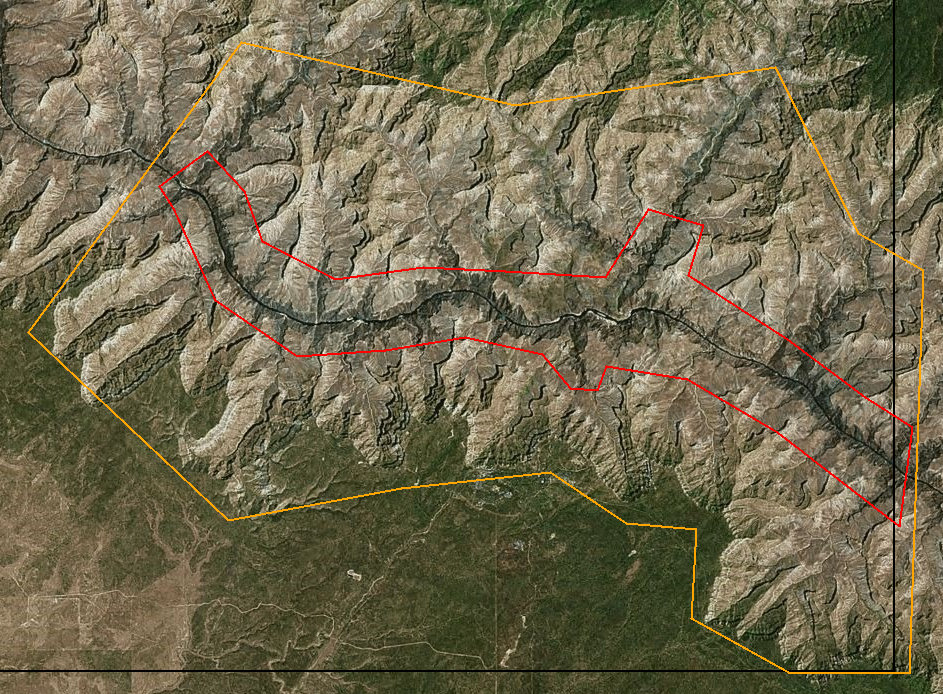
\includegraphics[width=16cm]{Images/grand_canyon_select.png}
\caption{\label{fig:grand_canyon_select}Example ZL choice in Grand Canyon}
\end{center}
\end{figure}
\end{center}
Also, if you wish to change Preview provider and/or zoomlevel for Preview, without loosing the polygons that you have already encoded, push ``Save and exit'', then go back with the ``Choose custom zoomlevel'', select your new choice and you should recover your polygons at the right position.

\bigskip

We go on with Step 1 as we have already learned, and since there isn't quite much OSM data past the Colorado river we may as well choose Min\_area=0, but for the same reason it wouldn't change much either to stick with the default value of 0.01.

\medskip

The important choice comes at Step 2 where we need to decide about the value allocated to {\tt Curv\_tol}.
Surely the Canyon is bumpy, and we should be tolerant enough. A general rule when bumpy terrain is suspected is to start with a value of 3, which will then be adapted if needed.
We next click the ``Custom DEM'' checkbox and use the file chooser to select our custom made {\tt N36W113.tiff}.
Step 2 button then performs his job and provides us with a mesh with 1.848.556 (the actual number may vary slightly when you'll try it yourself because the meshing algorithm contains some randomness), whose density is depicted (only in some small part) here below in Figure \ref{fig:grand_canyon_nodes1}.

\begin{center}
\begin{figure}[!ht]
\begin{center}
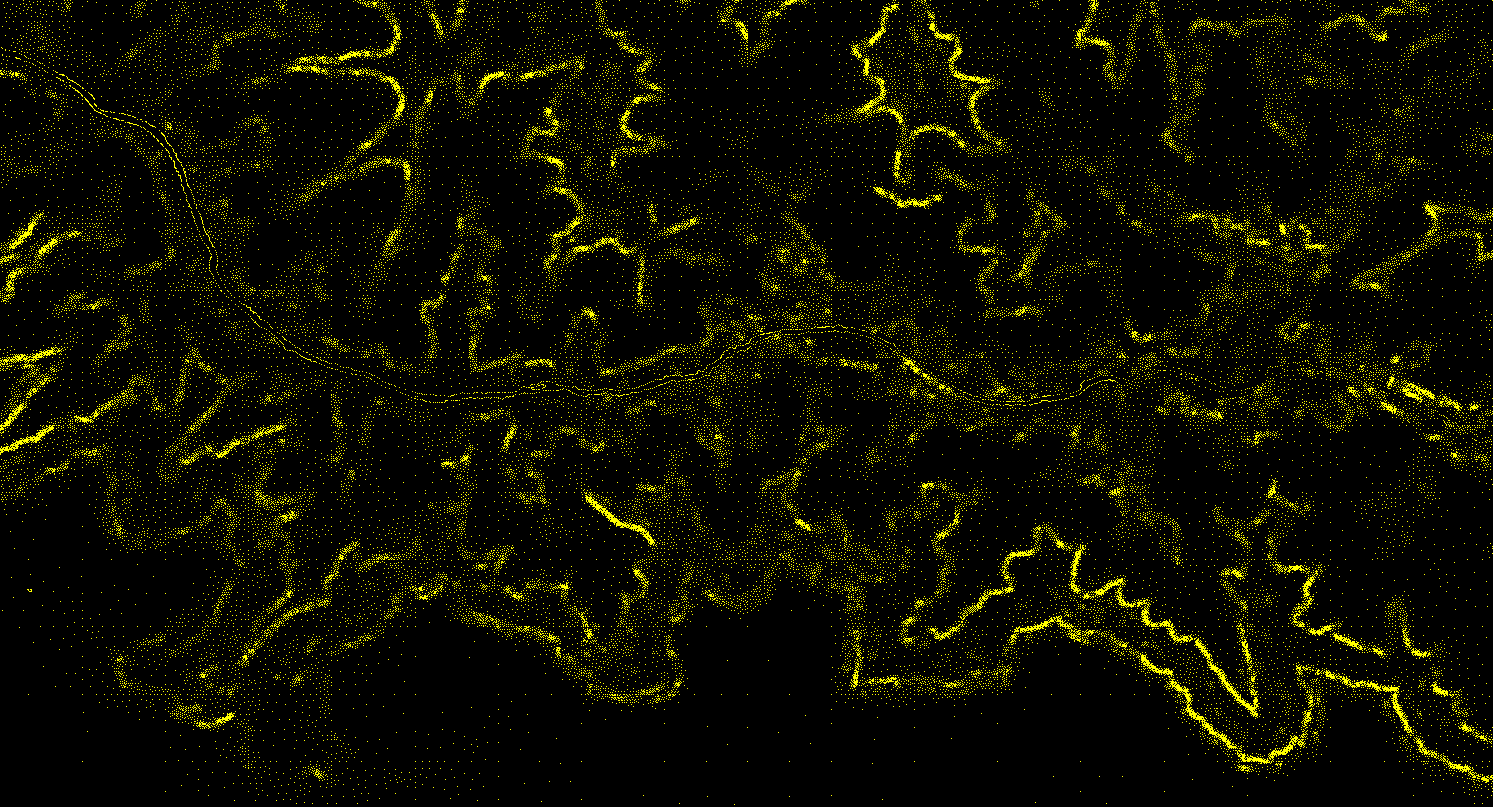
\includegraphics[width=16cm]{Images/grand_canyon_nodes1.png}
\caption{\label{fig:grand_canyon_nodes1}Density of Mesh points for Curv\_tol = 3}
\end{center}
\end{figure}
\end{center}

The UHD meshes of Alpilotx contain something like 3.5 million triangles per tile, and here we wish to push the limits a little bit to see how much we can grab from our detailed DEM (the later has 3*3600 to the square input points, which is roughly 100 millions! - but only a small proportion of these really have value, those that are in the Canyon and not the ones on the plateau). So we decrease the value of {\tt Curv\_tol} say to 1.5 and once more press the Step 2 button. Still not in accordance with our present braveness... Only when we finally reach {\tt Curv\_tol=0.5}, the value of 5 Millions triangles start to make us doubtful, and we shall stop here for today.

\begin{center}
\begin{figure}[!ht]
\begin{center}
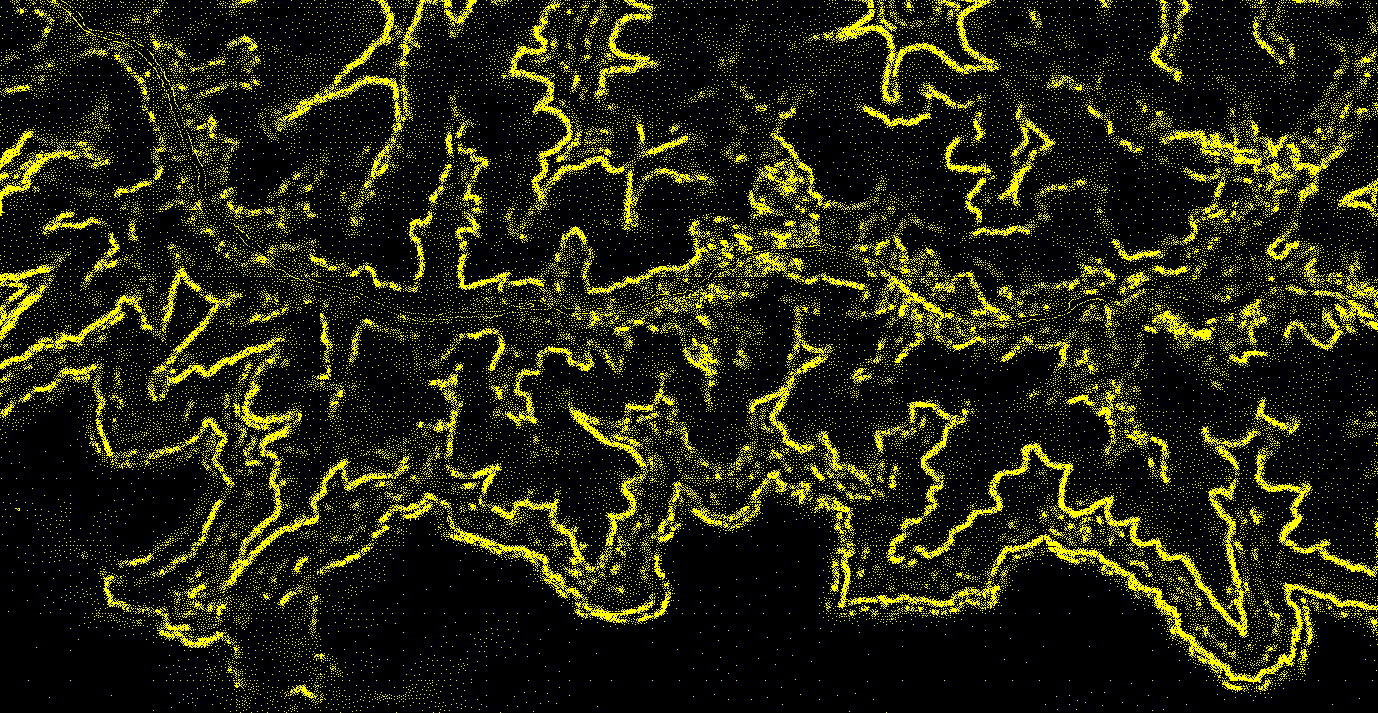
\includegraphics[width=16cm]{Images/grand_canyon_nodes2.png}
\caption{\label{fig:grand_canyon_nodes2}Density of Mesh points for Curv\_tol = 0.5}
\end{center}
\end{figure}
\end{center}

We finally press the Step 3 button (no masks are needed on this tile which do not contain any coastline).  After completion, perhaps we will meet playing the fool inside the Canyon ;-)  \href{http://www.youtube.com/watch?v=PFIcVbeHX7w}{http://www.youtube.com/watch?v=PFIcVbeHX7w}

\section{Sloped runway in the Alps}\label{alps}

The aim of this section is to present another functionality which we haven't used up to now : patch files. This feature will probably be (blindly) used by most of the users when flying in mountainous regions, but only few of them will probably embark in building their own patch (although, as the video below will show, the process is quite simplified by JOSM). The developers of 3D sceneries are hence the primary target of this section.

Not all airports have a flat runway in real life, and some of them are really far from.
Typical examples are Courchevel (LFLJ) and L'Alpe d'Huez (LFHU) in France, whose runways are sloped and rounded.

The reproduction of these two airports, either in the Global Scenery or in most of its higher density extensions, are missing some of the special features which characterize them. Similarly, without a patch file the mesh obtained using Ortho4XP for sloped airways would be either completely flat (e.g. LFLJ and LFHU, since their boundary is well defined in OSM), or absurdly bumpy (because most DEM file suffer from acquisition noise, an even without it wouldn't be able to reproduce at sufficiently small scale the roundedness).

{\bf Patch files come into play at the level of Step 1}, and therefore they play a similar role as OSM do in defining some closed polygons which are to be assigned with tags.
Whereas a closed way of water is assigned a tag telling whether it is inland or sea water, a patch defined through a patch file for a sloped runway will be tagged (within JOSM) by its {\tt altitude\_high}, {\tt altitude\_low} (and optionally by its {\tt profile}, {\tt steepness} and {\tt cell\_size}).
Even more simply, a patch whose aim is to flatten a piece of land will just be tagged by its target {\tt altitude}. The latter can be particularly useful in sloped terrain so that buildings are not flying over the ground  with just one corner touching.

Patch files are automatically processed by Ortho4XP when present in the {\tt Patches} subdirectory, corresponding to their Latitude/Longitude, provided their filename has the suffix {\tt .patch.osm}.
A small number, in particular those for LFHU and LFLJ, are already present in the 7z archive. They may be adapted freely, and developers of 3D sceneries who wish so are in particularly welcome to provide the community with patch files suited to their creation. Note that patches do not need to be related in any way to an airport, and can be used to flatten any polygonal area\footnote{provided it does not intersect transversally another patch, in particular a water patch!}, e.g. an airport otherwise not encoded in OSM (patch is local and yours, so it can be quite approximate, whereas when uploading data to OSM you should be much more careful).

Making a real-time video of the process was found to be easier (certainly to do but perhaps also to understand) than this manual. The one for LFHU can be found here :
\begin{center}
\href{http://www.youtube.com/watch?v=4Q3q5Lq4Kis}{http://www.youtube.com/watch?v=4Q3q5Lq4Kis}
\end{center}
and snapshots for the comparison before/after are in the two figures on the next page.\pagebreak

\begin{center}
\begin{figure}[!h]
\begin{center}
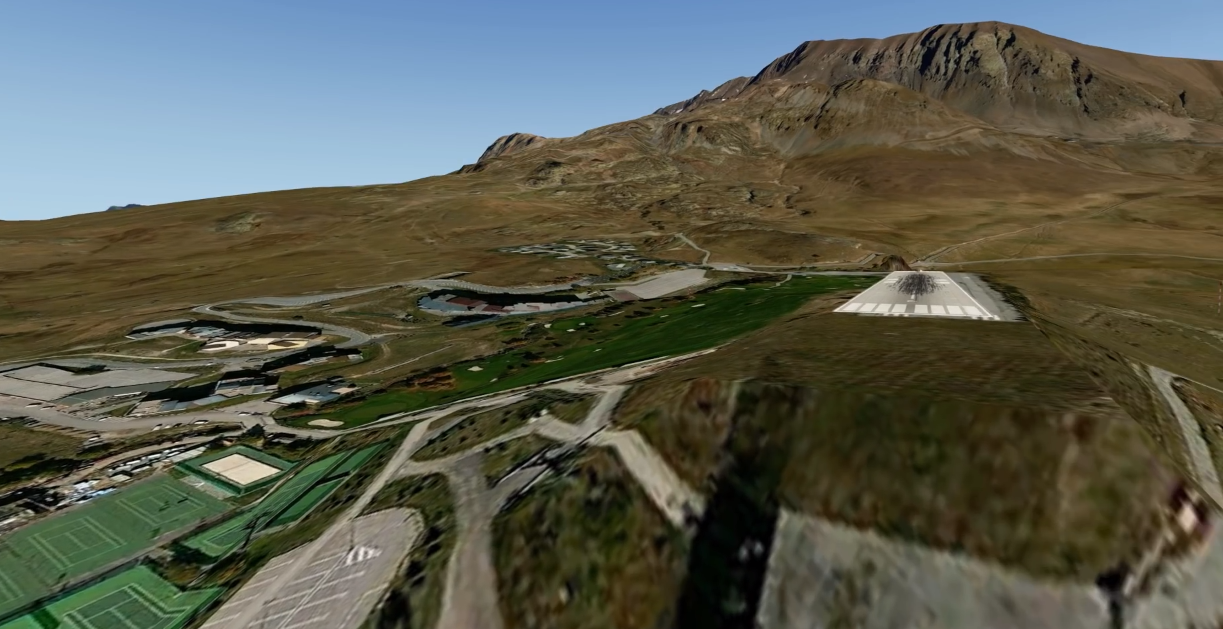
\includegraphics[width=16cm]{Images/LFHU_before.png}
\caption{\label{fig:LFHU_before}LFHU without patch is wrongly flattened}
\end{center}
Note that not only the runway is flat in the first image, but also that the parking and part
of the tennis courts are instead sloped !
\end{figure}
\end{center}
\begin{center}
\begin{figure}[!ht]
\begin{center}
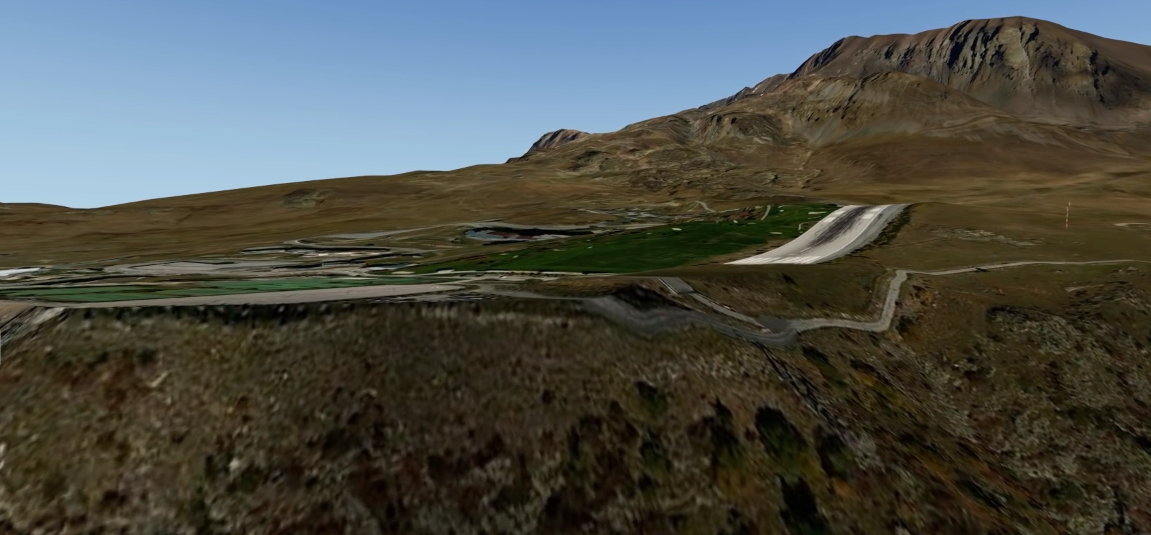
\includegraphics[width=16cm]{Images/LFHU_after.png}
\caption{\label{fig:LFHU_after}LFHU with a patch}
\end{center}
This second one looks more natural, and 3D objects will be welcome to give a bit of life to this wonderful but otherwise dull landscape! (and X-Plane does not have the runway exactly at the right position but that can be corrected independently)
\end{figure}
\end{center}

A more tricky example is the one for La Montagne Noire (LFMG) - not in the Alps but in the South-West of France not very far from Toulouse\footnote{Thanks to Daniel\_L for letting us discover this really nice airport!} - because of the hole for gliders just down the hangar, and since runways are crossing each other.  A video showing the result can be found here
\begin{center}
\href{\tt http://www.youtube.com/watch?v=vNawoSZEnyo}{http://www.youtube.com/watch?v=vNawoSZEnyo}
\end{center}
where the 3D scenery of LFMG is a creation of {\it Jean} available at {\tt xpfr.org}.
The following is an image of the patch for LFMG drawn in JOSM:
\begin{center}
\begin{figure}[!ht]
\begin{center}
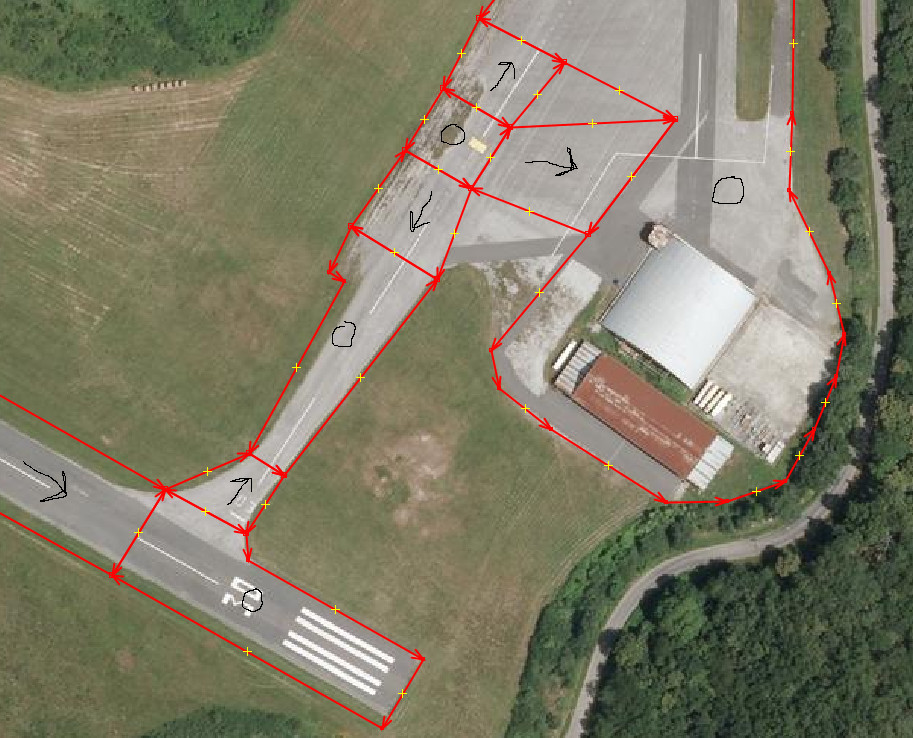
\includegraphics[width=16cm]{Images/LFMG_patch.png}
\caption{\label{fig:LFMG_patch}LFMG patch viewed in JOSM}
\end{center}
The zones where a zero was added are flattened, whereas the ones with an arrow are encoded
as sloped runway, the arrow representing the direction of climb.
\end{figure}
\end{center}

\begin{center}
\begin{figure}[!ht]
And we finish by a picture of Courchevel with its patch, where unfortunately we won't have
any snow in our orthophotos...     \begin{center}
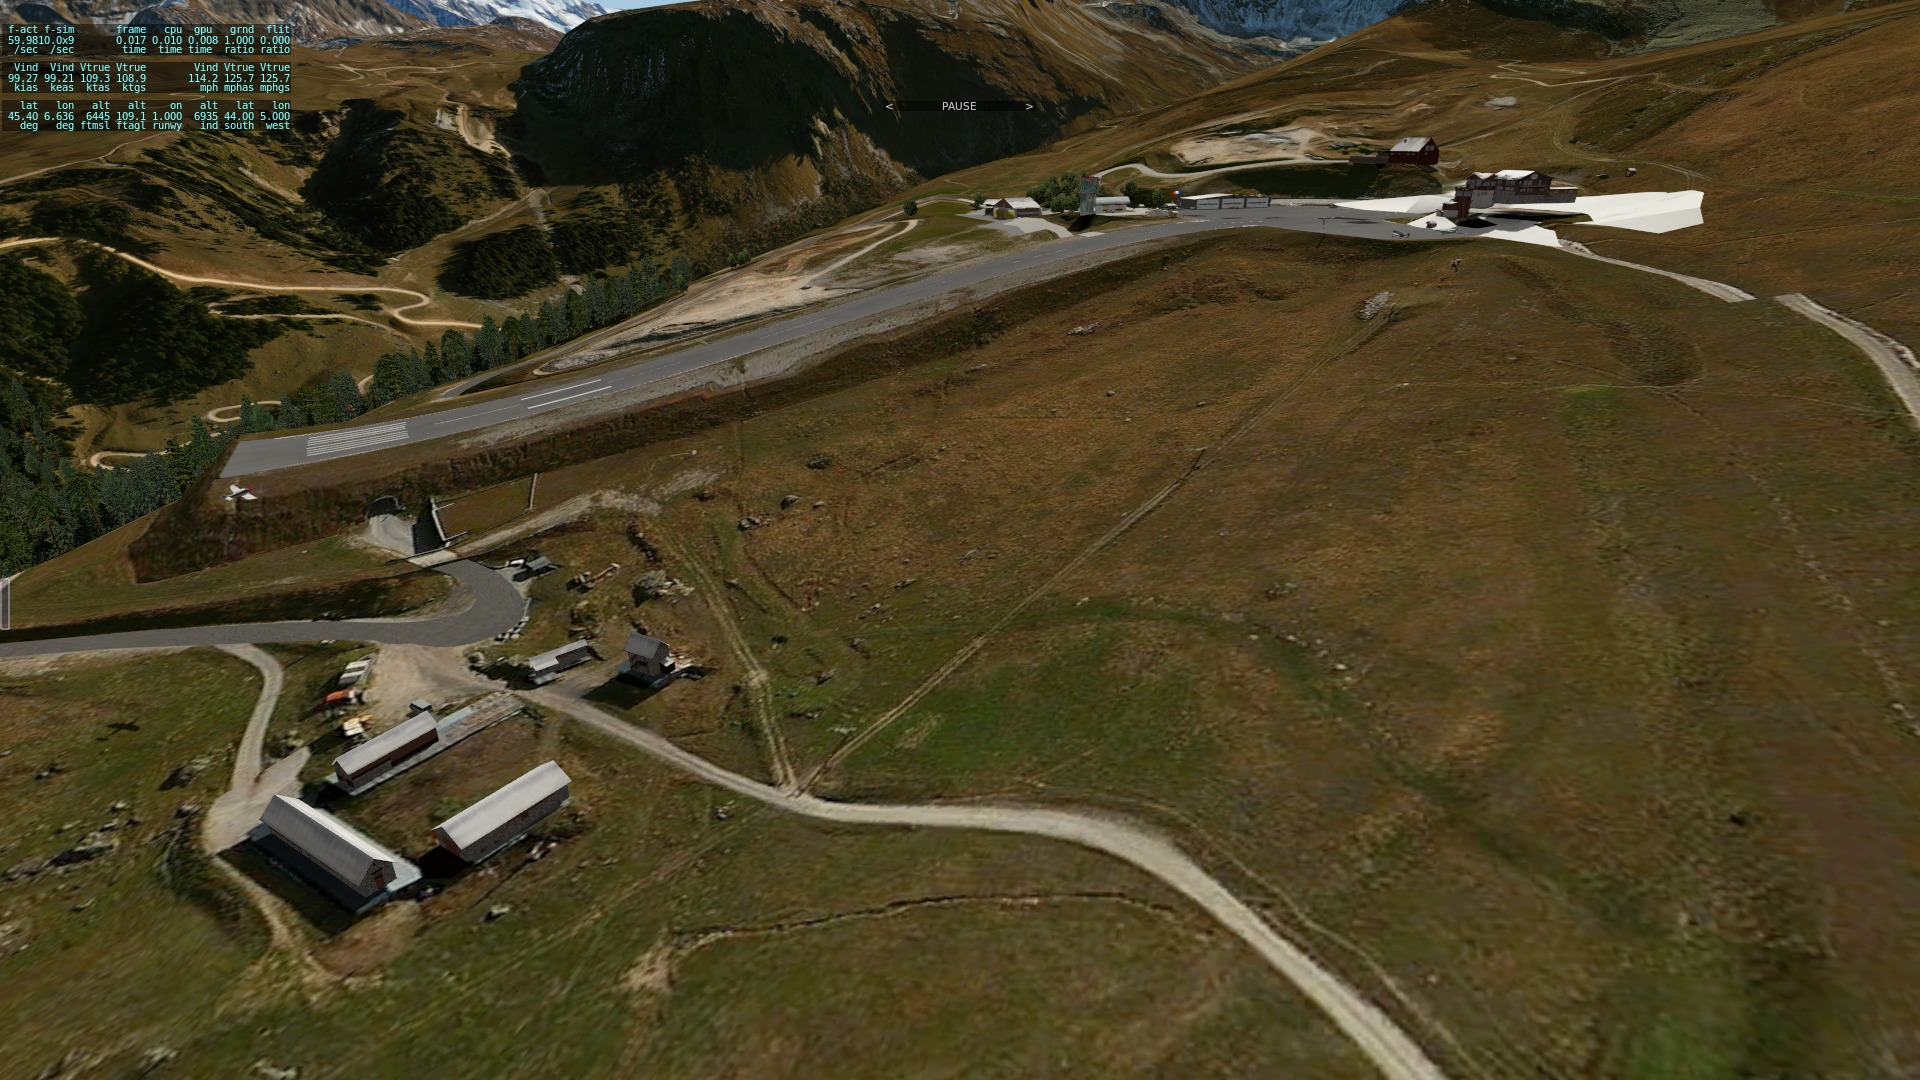
\includegraphics[width=16cm]{Images/LFLJ_overview.png}
\caption{\label{fig:LKJ_overview}LFLJ overview after the patch}
\end{center}
The tiny bits of snow high on the airport, as well as all the buildings, are objects part of a scenery by {\it Sky One} available on {\tt X-Plane.org}. The original scenery also comes with its proper mesh, here only the objects were used as is.
\end{figure}
\end{center}

There are two important rules that are worth noting here :
\begin{itemize}
  \item
  {\bf Sloped runways should be encoded with four points only, the first point should be one of
  the two points on the highest lateral side, and the second point is the one opposite to him on the low side.}
  \item
  {\bf If a polygonal patch to be flattened (say an apron) is to be linked to a sloped runway,
  the linking has to be along a lateral side of the runway, and matching exactly that lateral
  side (it is indeed not conceivable to match a flat edge with a sloped one...).}
\end{itemize}


\section{Reference/technical notes}


\subsection{Water options}
\begin{enumerate}
  \item X-Plane only. Patches of water that are kept in Step 1 are textured only with X-Plane original water. Those that are not kept (e.g. if {\tt Min\_area} is non zero) will appear as orthophotos.
  
  \item  Orthophoto only. The sea water appears as X-Plane water, but all inland water is orthophoto only. You should make Step 1 {\it after} checking this option, since all inland water edges will then be omitted.
  \item Mixed : {\tt ratio\_water} is a real value between 0 and 1, correspond to the ratio between orthophoto water and X-Plane water. Close to zero the orthophoto is dominant, and conversely.  The default value is 0.2.\\
  {\it Hint:} The scale is read in the gradient file {\tt water\_transition.png}, modifying this file within the tile allows to avoid rebuilding the DSF in case you changed your mind.
\end{enumerate}
\subsection{Sea\_equiv}
This list, which is to be defined in the config file {\tt Ortho4XP.cfg}, contains the OSM names
(these need to be exactly the ones of the OSM `rel' equivalent) of big patches of water which you would like to see treated as if they were sea water (and hence get an automatic mask of a certain width rather than a constant alpha channel).
The reason for this list is that for very big lakes (like Lake L\'eman) as for the sea, the orthophotos are not always usable on their whole surface.

\subsection{Custom and base Zoomlevels}
The set of couples (zone,zoomlevels) is turned eventually into an ordered list. The last element in this list is always the one corresponding to the choice on the main window, not on the preview
window. The ones encoded in the preview window are ordered by decreasing zoomlevel (in case the zoomlevels are identical the encoding order is preserved for the subclass). When a triangle of the mesh needs to be attributed a texture, each zone is checked for inclusion, beginning  from the first one and until one is found.
If none is found from the Preview zones, the ZL and provider from the last zone (which corresponds the main window and hence to the entire tile) will be used. Notice that the ``Base source'' listbox contains the entry 'None'. If this is used, and a triangle finds no zone in the Preview list, it will be attributed a generic X-Plane texture (namely {\tt lib/g10/terrain10/fruit\_tmp\_wet\_hill.ter}). Encoding of polygons in the Preview window is done with by "shift+click" or "p", the last encoded point can be removed with "backspace", and each zone should be finished by clicking the "save zone" button, including the last one prior to pushing the "ave and exit" button. The best way to learn is probably to practice here...


\subsection{Min\_area}
Each closed OSM way of water is tested for his size. If the latter is greater than {\tt Min\_area} (in $km^2$ unit), it is kept, otherwise it is discarded and will only appear as water orthophoto.
The fact is that small patches of water do not always benefit a lot from the transparency effect,  and on the other hand a few OSM errors can sometimes be circumvented by a larger value of {\tt Min\_area} simply because the faulty ways are let aside due to their small size.
Typical values are $0$ (for the brave), $0.001$ (for me) and $0.01$ (for the careful). Note that $0.001$ is basically the size of a swimming-pool.

\subsection{Curv\_tol / Min\_angle}
{\tt Curv\_tol} stands for tolerance to curvature. The lower its value, the higher the complexity of the mesh and the number of triangles it contains.  A safe rule {\it when experimenting your first tiles}\footnote{After a while you will be spot on at the first try! Of course flat island tile allow for smaller values of {\tt Curv\_tol} than the Himalaya or the Alps.} is to start
with {\tt Curv\_tol=3}, try to launch Step 2 and read the number of triangles it generates (``Mesh triangles'' indicated with arrows in the terminal pane). If that number is substantially lower than your target, decrease {\tt Curv\_tol} (say by a factor 1.5 or 2), and on the contrary increase it. You can repeat the operation as many times as you like.\\
{\bf So what is a good value of target total mesh triangles ?} Well, first it depends whether the tile has plenty of sea water or not, since the latter should almost count as zero for the triangle count. Therefore keep in mind to always scale the numbers as if the tile was without water. Once this is known and taken into account, it is a matter of taste/cpu/etc : just for comparison a Global Scenery tile has roughly 500.000 triangles, and HDv3 one 1.5 million and a UHDv1 one 3.5 millions. I have tested tiles with almost 10 millions triangles on my 8Gb RAM computer, without noticeable impact at runtime, but these are longer to construct too and most
of the time I am happy with something between 1 and 3 million triangles. \\
{\tt Min\_angle} as its name indicates is a target minimum smallest angle for each triangle. This is only a target (one cannot fill a small OSM angle with suitable triangles if {\tt Min\_angle} is larger than that angle), and in any case it should be kept not too big (the default value is 5 degree if you check the box, and 35 is a value for which the algorith will surely {\it not} terminate). It is only really meaningful with patches since it has some impact on the way say a flattened patch will be linked back to the DEM points outside (with a zero or very small {\tt Min\_angle} the transition can be rough, which you can want or want to avoid depending on cases).

\subsection{Custom DEM}
\begin{enumerate}
  \item They should be in Geotiff or HGT format
  \item They should have the same number of column and rows
  \item Their corners should coincide exactly with the corners of the 1x1 degree tile.
\end{enumerate}
If not using Custom DEM but ``default'' ones are used. These need however to be downloaded by yourself prior to building a tile. The default two locations for download and the naming scheme is described precisely at the very beginning of Section \ref{grandcanyon}.

\subsection{Skip downloads/converts}
If --for some reason-- you do not want to download the textures but just to build the DSF, use {\tt Skip downloads} (it enforces {\tt Skip converts} too). I you wish to download, but want to leave the conversion from jpeg to dds to a future time (perhaps because you want to process/improve the jpegs first), use {\tt Skip converts}. Note that conversion (since it is presently not multi-threaded) is often the bottleneck regarding process time (4sec per 4K texture roughly, whereas download and montage can be as quick as 1sec per 4K texture with the big providers).

\subsection{User defined vs Automatic masks}
Automatic masks follow a naming scheme related to TMS orthophotos at ZL14 (actually Google version of it, see e.g. \href{http://www.maptiler.org/google-maps-coordinates-tile-bounds-projection/}{http://www.maptiler.org/google-maps-coordinates-tile-bounds-projection/} for a nice explanation of these numberings).
If you want to build your own masks (the automatic process does not know where he could use more or less of the offshore orthophotos) you just  need to use the same filename but append it with and underscore followed by the provider acronym, like say 5664\_7952\_FR.png or 5664\_7952\_BI.png in place of 5664\_7952.png. They will then be used in priority over the automatic ones if both are found.

\subsection{Read/write Config}
See Ortho4XP.cfg below. You should only push the ``Write config'' button if you started
encoding detailed polygons in the Preview and the milkman suddenly knocked the door, it is otherwise automatically called by ``Build tile''. You should only push ``Read config''
if you wish to update or improve a tile that you have already (at least partially) built and which is present in Ortho4XP base dir.


\subsection{Stop process (cleanly)}
As its name suggests, it strives to stop cleanly a process that, for some reason, the user would like to stop (wait for the messages from all the threads!). Instead, not doing so and stopping it through e.g. a CTRL-C would probably lead at least to a non empty tmp directory and at worse to corrupted image files.

\subsection{Ortho4XP.cfg}
The file Ortho4XP.cfg is a python source file as well, and it is executed at the very beginning of Orhto4XP. In particular, it must follow Python's syntax.\\
With the help of the graphical interface, users should not need to edit the config file on a regular basis.
Only the values of the colorimetry corrections dictionary for the different providers, the list
${\tt sea_equiv}$, and some file locations are found in Ortho4XP.cfg and only in Ortho4XP.cfg.
When a tile is built, it contains its proper version of Ortho4XP.cfg obtained by concatenation of the global Ortho4XP.cfg file with the input from the graphical interface (in particular the polygons of the Preview window if such were defined).\\
If Ortho4XP is launched, lat/lon are selected and the ``Read config'' button is pressed, the data
saved in that prior tile (it if exists) is reloaded in the interface.

\subsection{Carnet\_d\_adresses.py}
This is {\it your} address book of providers. You may extend it, share it with your friends or keep it secretly. In any case, since we are not really invited but only tolerated, we should pay attention to not cutting the branch on which we all sit.

\section{Caveats/F.A.Q.}
\subsection{My airport has bumpy runways}
This mean that it hasn't been flattened, and his name or ICAO code did not appear when you performed Step 1. There are two ways to get it flat.  The first one is to encode its boundary as a closed way on OSM (don't forget to add the tag "aeroway"="aerodrome", then (optional but recommended) one tag for its name and one for its ICAO code).  Pay attention to reuse as much as possible existing OSM nodes, and to close the way. Also, if the airport is nearby some water patch, do not make it cross those edges, or you will come back with the error \ref{crash}.
The second solution is to build a patch file with just one polygon surrounding the airport and indicated with the altitude tag of the airport.  An example of such a patch is contained in the 7z archive for Paris Orly airport (LFPO), it was made using JOSM as in the LFHU video in Section \ref{alps}.

\subsection{Part of my new tile is flooded with water}
In OSM, the oriented broken line which defines the coastline should always have the water on its right. To determine which triangles need to be tagged as sea triangles, you can imagine that Ortho4XP let a drop of ink on the (supposedly) correct side of the coastline and let it contaminate nearby triangles as long as it is not blocked by the coastline. If some part of the coastline is mistakenly oriented, the drop of ink falls on the ground and then makes its way inland...
Correction in OSM is the only viable cure.

\subsection{Step 2 will not terminate or with an error :-(}\label{crash}
In rare circumstances Step 2 can take longer than a minute, but in most it should finish in a few tens of seconds. If you have asked for a {\tt Min\_angle}, try first without it (this requirement is sometimes difficult to satisfy depending on the OSM data). If it still can't terminate, with a very high probability it is again related to an error in OSM, and Triangle4XP may even indicate to you where you should look for it.
This may happen when two edges in OSM do cross each other in a different point than their end-points (it should never be so in principle, but Open also means open to mistakes).
In most cases, this is due to a small part of a river that has been encoded twice, or patches of water that are not ``glued'' together the appropriate way. With a little bit of experience one can find and correct them directly online, but in rare cases it can turn into a ``treasure'' hunt.

\subsection{Step 3 complains about no place left in the pool !}
This means that the mesh would have more than 65536 points in the equivalent of a ZL17 texture.
This can be caused either by an OSM error (causing the mesh tool to become mad there), or to a value of {\tt Curv\_tol} too small. Try first with {\tt Curv\_tol=3}, if the problem persists the issue is on OSM, correct it or report it and somebody will look for you.

\subsection{Help! Do I need to erase my tile and resume from start ?}
No ! Radical decisions are rarely productive. If you have downloaded orthophotos and if they look correct when viewing them you should certainly not erase them because some other unrelated part is causing trouble.
More generally I known of only two cases where one would need to erase something~:
\begin{enumerate}
  \item A network problem at your place has caused some orthophotos to be corrupted (these do not show in a file viewer or make a viewer crash). Then simply erase those that appear corrupted. If the issue is on the server side, Ortho4XP will keep trying and will not build corrupted images.
  \item An error was found on Openstreetmap that was causing troubles to Triangle4XP in Step 2.
  Then after correction on OSM you should erase the cached OSM data on your disk, this is the object of the button ``Purge OSM data'' which you should only use in that case (or because OSM data has been updated).
\end{enumerate}
\subsection{A few orthophotos are corrupted with white squares.}
Typically 256x256 or 2048x2048 of size. This is due to a (slow) server that was probably overloaded.  When this happens, they can sometimes send white data without necessarily noticing. I some cases we wish to keep these (and this is not due to overload but to missing data, e.g. in boundary textures of providers whose data do not go beyond the border), in the other cases one solution is to erase the corrupted orthophotos and to build the tile once more so that (only) the deleted ones will be (re)downloaded (hopefully correctly).
The sources 'CH\_Vs', 'NZ' and 'NO' have sometimes showed this kind of behaviour when used from France.

\section{Acknowledgements}
My greatest ``Mercis!'' to all the members of the french forum x-plane.fr whose help and encouragements have been a great source of motivation since June this year when an early development version was first released there. Many of the features included in the present version have emerged from their remarks and ideas, and it should now really be considered a collective work. The list would be too long to name them all, in exchange and since a non trivial proportion of them are belgian, I owe them all a big glass of Beer4XP. Many thanks also to Pascal from zonephoto.x-plane.fr, to Peter (Durian) from x-plane.org and to Tony (tonywob) from avsim.com, with whom interaction has always been fruitful.

\smallskip

\noindent Many thanks also to the two Jonathan.\\
- Jonathan Shewchuk for his impressive``Two-Dimensional Quality Mesh Generator and Delaunay Triangulator'', {\it Triangle}, which is so powerful and flexible that it wasn't a hard task to turn it into a 2.5D mesh generator for our X-Plane tiles, and since 99\% of Triangle4XP is indeed really {\it Triangle} itself.\\
- Jonathan de Ferranti for his impressive work of building high quality digital elevation models (DEM) and for letting them accessible on his viewfinderpanorama website.

\smallskip

\noindent The expertise of Ben Supnik and Andras Fabian has also been much appreciated at the early stage of the project when trying to understand the peculiarities of X-Plane scenery files. I have not convinced them that such a mesh-tool would be interesting as well for building land-class based sceneries, but the debate remains open ;-)

\medskip

\noindent Finally, my warmest thanks (and apologies) to my wife and daughters, who have resisted many times throwing my computer through the window when they could have done so.
\end{document}
